\documentclass[letter,12pt]{article}
\usepackage[T1]{fontenc}
\usepackage[utf8]{inputenc}
\usepackage{lmodern}
\usepackage{hyperref}
\usepackage[english]{babel}
\usepackage{fourier}
\usepackage[protrusion=true,expansion=true]{microtype}
\usepackage{amsmath,amsfonts,amsthm}
\usepackage[pdftex]{graphicx}
\usepackage{sectsty}								
\usepackage[svgnames]{xcolor}			
%\allsectionsfont{\centering \normalfont\scshape}	
\usepackage{fancyhdr}
\pagestyle{fancyplain}
\fancyhead{}	
\fancyfoot[L]{\small \url{http://toddvance.tech}}		
\fancyfoot[C]{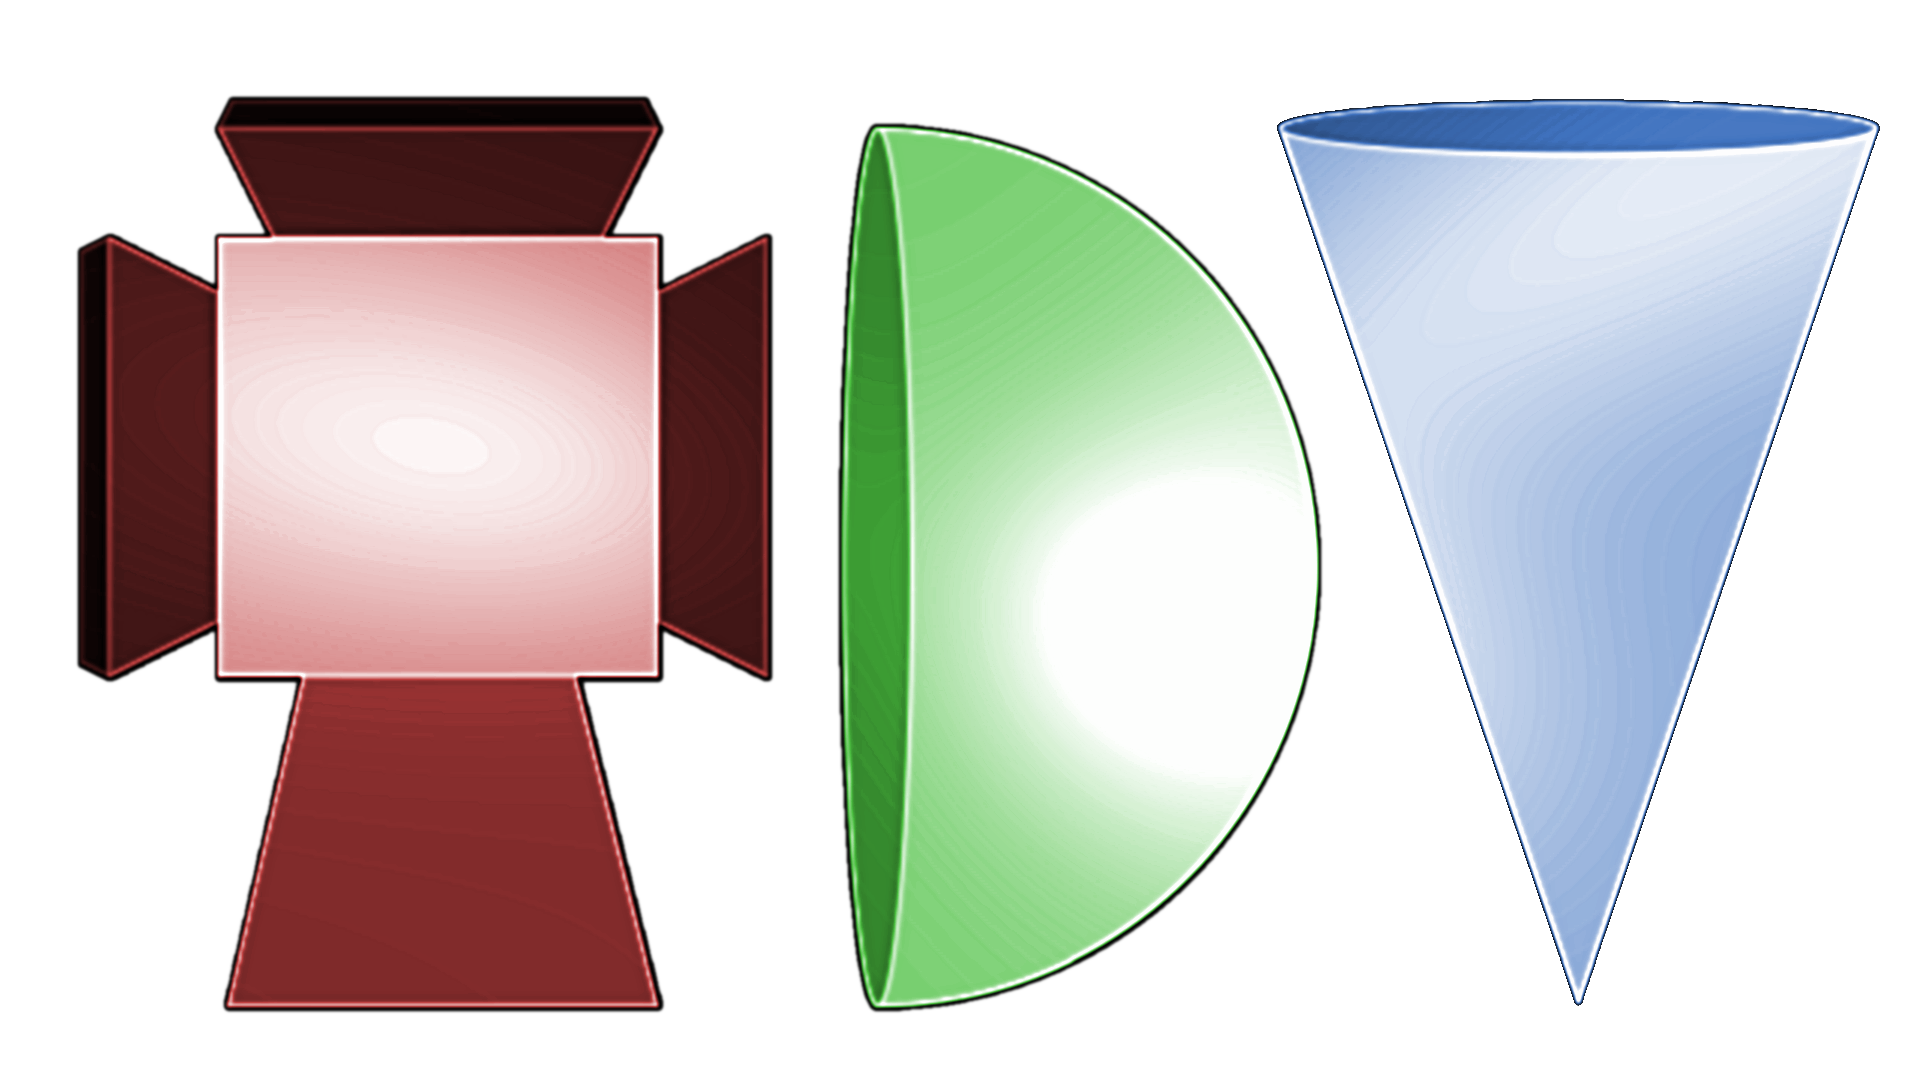
\includegraphics[width=0.5in]{common/monogram-transparent.png}}											
\fancyfoot[R]{\thepage}								
\renewcommand{\headrulewidth}{0pt}			
\renewcommand{\footrulewidth}{0pt}
\setlength{\headheight}{13.6pt}
\newcommand{\horrule}[1]{\rule{\linewidth}{#1}} 	% Horizontal rule

\title{
		%\vspace{-1in}
		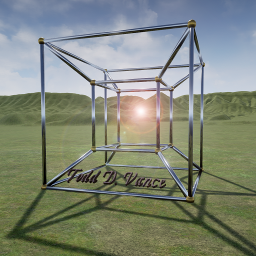
\includegraphics[width=1.5in]{common/tdv-logo-south-branch-valley-small.png}
		\usefont{OT1}{bch}{b}{n} 
		\normalfont 
		\horrule{0.5pt} \\[0.4cm]
		\Huge Unreal Engine 4 Notes\\ %%%%%%%%%%%%%% TITLE %%%%%%%%%%%%%%%
		\color{DarkGreen}
		\large How To\\[0.2cm]%%%%%%%%%%%%%%ARTICLE TYPE %%%%%%%%%%%%%%%
		\color{Blue}
		\small \textsc{Udemy “Learning To Code By Making Games in Unreal 4” course}\\%%%%%%%%%%%%%% TAG LINE %%%%%%%%%%%%%%%
		\color{Black}
		\horrule{2pt} \\[0.5cm]
}
\author{
		\normalfont \normalsize
       \copyright{2017 Todd D. Vance, Deplorable Mountaineer}%%%%%%%%%%%%%% COPYRIGHT %%%%%%%%%%%%%%%
        \tiny\\
\tiny        Permission is hereby granted, free of charge, to any person obtaining a copy\\[-0.3cm]
\tiny        of this software and associated documentation files (the "Software"), to deal\\[-0.3cm] 
\tiny        in the Software without restriction, including without limitation the rights to\\[-0.3cm]
\tiny         use, copy, modify, merge, publish, distribute, sublicense, and/or sell copies\\[-0.3cm] 
\tiny         of the Software, and to permit persons to whom the Software is furnished to\\[-0.3cm]
\tiny         do so, subject to the following conditions:\\[-0.3cm]
\tiny         \\[-0.3cm]
\tiny	The above copyright notice and this permission notice shall be included in all\\[-0.3cm]
\tiny	copies or substantial portions of the Software.\\[-0.3cm]
\tiny	\\[-0.3cm]
\tiny	THE SOFTWARE IS PROVIDED "AS IS", WITHOUT WARRANTY OF ANY KIND,\\[-0.3cm]
\tiny	EXPRESS OR IMPLIED, INCLUDING BUT NOT LIMITED TO THE WARRANTIES\\[-0.3cm] 
\tiny	OF MERCHANTABILITY, FITNESS FOR A PARTICULAR PURPOSE AND\\[-0.3cm]
\tiny	NONINFRINGEMENT. IN NO EVENT SHALL THE AUTHORS OR COPYRIGHT\\[-0.3cm]
\tiny	HOLDERS BE LIABLE FOR ANY CLAIM, DAMAGES OR OTHER LIABILITY,\\[-0.3cm]
\tiny	WHETHER IN AN ACTION OF CONTRACT, TORT OR OTHERWISE, ARISING\\[-0.3cm]
\tiny	FROM, OUT OF OR IN CONNECTION WITH THE SOFTWARE OR THE USE\\[-0.3cm]
\tiny   OR OTHER DEALINGS IN THE SOFTWARE.
}
\date{\today}

\newtheorem{exercise}{Exercise}

\begin{document}
\maketitle{}
\tableofcontents{}

%%%%%%%%%%%%%% BEGIN DOCUMENT %%%%%%%%%%%%%%%

\section{Unreal Notes}

Roughly in the order they come up in the Building Escape section.

\begin{enumerate}
\item My .gitignore, made to work in root directory at the expense of being extra aggressive:

\begin{verbatim}
**/*.VC.db
**/*.opensdf
**/*.opendb
**/*.sdf
**/*.sln
**/*.suo
**/*.xcodeproj
**/*.xcworkspace
**/Build
**/Binaries
**/ DerivedDataCache
**/Intermediate
**/Saved
**/StarterContent/
\end{verbatim}

\item F8 while playing to eject

\item alt + left mouse button: rotate around focused object (f to focus on selected object)

\item alt + right mouse button: zoom at focused object 

\item W, E, R to change translate/rotate/scale

\item Log with: 	UE\_LOG(LogTemp, Warning, TEXT("Begin: Position Report"));

\item Or with 	UE\_LOG(LogTemp, Warning, TEXT("Begin: Position Report on \%s"), *fstring);

\item Hold down L and doubleclick to place a point light

\item GetWorld() to search for scene objects

\item Find a player controller, then get pawn in order to get the player pawn.

\item GetWorld() has a GetTimeSeconds() method.

\item To open VS2015 on a component .h file, click object, left click its component in Details window to show its properties, then right-click that component instead to be able to select “open whatever.h”

\item UPROPERTY “macro decorator” takes things like EditAnywhere or VisibleAnywhere

\item Create a component: Content Browser -> Add New -> C++ file -> Actor Component

\item Create default pawn blueprint from the current default pawn: play game, eject, select player pawn in game,
go to Blueprints menu->convert selected actor to blueprint class

\item Create game mode blueprint from current game mode: Blueprints -> create empty blueprint class -> open all classes and find <name of game>GameModeBase class and select it.

\item Specify new game mode: project settings->maps and modes; and override in blueprints menu item.  In the game mode blueprint, ensure it has the right default pawn and recompile.

\item Specify default pawn for game mode: project settings->maps and modes and recompile the new default pawn blueprint.

\item Add component to default pawn: open its blueprint class and click Add Component.

\item Get player viewpoint: GetWorld()->GetFirstPlayerController()->GetPlayerViewPoint(OUT location, OUT rotation);

\item rotation.Vector() is the unit “forward” vector of a rotation

\item DrawDebugLine to draw a debug line between two locations

\item Check the SimulatePhysics checkbox on an actor instance, then set a reasonable mass, will make it moveable, etc. automatically.  You may still need to add a  collision to the mesh, though.

\item Setting up raytracing:

\begin{verbatim}
//Set-up Query Parameters
	FCollisionQueryParams CollisionQueryParams(FName(TEXT("")), false, GetOwner());

	// ray-cast to reach distance
	FHitResult HitResult;
	GetWorld()->LineTraceSingleByObjectType(OUT HitResult, location, LineTraceEnd, FCollisionObjectQueryParams(ECollisionChannel::ECC_PhysicsBody), CollisionQueryParams);
\end{verbatim}

\item Add physics handle component to default pawn to give it some interaction abilities (e.g. it has a GrabComponent method).  In code, it gets the class name 	UPhysicsHandleComponent. FindComponentByClass() to get the component, e.g.
\begin{verbatim}
	PhysicsHandle = GetOwner()->FindComponentByClass<UPhysicsHandleComponent>();
\end{verbatim}
\item Also, collision component should simulate physics, generate hit and overlap events.

\item Input Binding, action mappings, axis mappings (can be player remappable), call a function on input:
\begin{enumerate}
\item input component -- e.g. default pawn has a PawnInputComponent.  Stack of InputComponents managed by PlayerController.  Processed by PlayerInput.   Each component on a stack consumes an event, preventing further input componets from processing it.  Transient : only exists at runtime.

\item In code that is a component of the default pawn, get the physics handle component and the input component at begin play, and store them in fields of the class.

\item In ProjectSettings->Engine:Input, set desired actions/axes.  Note exact action names: must be spelled the same in the code.

\item In code, can bind the new action or axis to a method: InputComponent->BindAction(“exact action name”) for example.

\begin{verbatim}
		InputComponent->BindAction("Grab", 
		      EInputEvent::IE_Pressed, this, &UGrabber::Grab);
\end{verbatim}

\item Full grabber code:

\begin{verbatim}
// Copyright (C) 2017 Todd D. Vance

#include "BuildingEscape.h"
#include "Grabber.h"


#define OUT 

// Sets default values for this component's properties
UGrabber::UGrabber()
{
	// Set this component to be initialized when the game starts, and to be ticked every frame.  You can turn these features
	// off to improve performance if you don't need them.
	PrimaryComponentTick.bCanEverTick = true;

	// ...
}


void UGrabber::Grab()
{
	UE_LOG(LogTemp, Warning, TEXT("%s is grabbing"), *(GetOwner()->GetName()));

	UPrimitiveComponent *ComponentToGrab = CurrentHitResult.GetComponent();
	if (ComponentToGrab && HasHitResult)
	{		GrabbedObject = ComponentToGrab->GetOwner();
		PhysicsHandle->GrabComponentAtLocationWithRotation(ComponentToGrab, NAME_None, GrabbedObject->GetActorLocation(), GrabbedObject->GetActorRotation());
		UE_LOG(LogTemp, Warning, TEXT("%s is grabbing....%s"), *(GetOwner()->GetName()), *GrabbedObject->GetName());
	}
	else
	{
		UE_LOG(LogTemp, Warning, TEXT("%s is grabbing....nothing"), *(GetOwner()->GetName()));
	}

}


void UGrabber::Release()
{
	UE_LOG(LogTemp, Warning, TEXT("%s is releasing"), *(GetOwner()->GetName()));
	PhysicsHandle->ReleaseComponent();
	GrabbedObject = nullptr;
}


// Called when the game starts
void UGrabber::BeginPlay()
{
	Super::BeginPlay();

	UE_LOG(LogTemp, Warning, TEXT("Begin: Grabber on %s"), *(GetOwner()->GetName()));
	PhysicsHandle = GetOwner()->FindComponentByClass<UPhysicsHandleComponent>();
	if (!PhysicsHandle)
	{
		UE_LOG(LogTemp, Error, TEXT("No Physics Handle Component on %s"), *(GetOwner()->GetName()));
	}

	InputComponent = GetOwner()->FindComponentByClass<UInputComponent>();
	if (!InputComponent)
	{
		UE_LOG(LogTemp, Error, TEXT("No Input Component on %s"), *(GetOwner()->GetName()));
	}
	else
	{
		///bind input action
		InputComponent->BindAction("Grab", EInputEvent::IE_Pressed, this, &UGrabber::Grab);
		InputComponent->BindAction("Grab", EInputEvent::IE_Released, this, &UGrabber::Release);

	}


}


// Called every frame
void UGrabber::TickComponent(float DeltaTime, ELevelTick TickType, FActorComponentTickFunction* ThisTickFunction)
{
	Super::TickComponent(DeltaTime, TickType, ThisTickFunction);

	// Get player viewpoint this tick
	FVector location;
	FRotator rotation;
	GetWorld()->GetFirstPlayerController()->GetPlayerViewPoint(OUT location, OUT rotation);
	/*UE_LOG(LogTemp, Warning, TEXT("Viewpoint: location=%s, rotator=%s"),
		*(location.ToString()), *(rotation.ToString()));*/

	FVector LineTraceEnd = location + rotation.Vector()*Reach;
	//DrawDebugLine(GetWorld(), location, LineTraceEnd, FColor(255, 0, 0), false, 0, 0, 5);

	//Set-up Query Parameters
	FCollisionQueryParams CollisionQueryParams(FName(TEXT("")), false, GetOwner());

	FHitResult HitResult;

	// ray-cast to reach distance
	// see what we hit
	HasHitResult = false;
	if (GetWorld()->LineTraceSingleByObjectType(OUT HitResult, location, LineTraceEnd, FCollisionObjectQueryParams(ECollisionChannel::ECC_PhysicsBody), CollisionQueryParams))
	{
		//UE_LOG(LogTemp, Warning, TEXT("HitResult: %s "), *(HitResult.GetActor()->GetName()));
		CurrentHitResult = HitResult;
		HasHitResult = true;
	}
	
	if (PhysicsHandle->GrabbedComponent)
	{
		PhysicsHandle->SetTargetLocation(location);
	}

}
\end{verbatim}
\end{enumerate}

\item: Iterate over every actor in the world:

\begin{verbatim}
for (TActorIterator<AActor> ActorItr(GetWorld()); ActorItr; ++ActorItr)
	{
		AActor* Actor = *ActorItr;
		//do stuff
	}
\end{verbatim}

\item Expose any “code” object to blueprint: select object, then Blueprints->convert selected actors to blueprint.  Note any other instances of the object you want as blueprint, you have to replace them with the blueprint version.  Note, you have to replace component properties linking to objects, as they will be cleared (and if you don’t have guard code, UE4 will crash on dereferencing the null pointer!)

\item Add Timeline action in blueprint Event Graph to add animation.

\end{enumerate}











\end{document}
